\chapter*{key mapping}
The following key map is the default for Subluminal when starting the game for the first time. You can change them via the ingame settings menu. The changes are stored persistently in the \textbf{config} folder and are protable.

%\begin{multicols*}{3}
\section*{general}
These key combinations are accesible during every game state.\\[0.5em]
\keystroke{S} : show settings \\[0.5em]
\keystroke{C} : show chat \\[0.5em]
\keystroke{F4} : toggle framerate \\[0.5em]
\keystroke{F5} : toggle framerate chart \\[0.5em]
\keystroke{F6} : toggle server tick \\[0.5em]
\keystroke{F7} : toggle server tick chart \\[0.5em]
\keystroke{F11} : toggle fullscrreen \\[0.5em]
  
\section*{menu / lobby}
This key combination is only available at the start of the game.\\[0.5em]
\Esc : skip intro\\[0.5em]

\section*{in-game}
These shortcuts are used to control the game.\\[0.5em]
\emph{Left Click} : select star \\[0.5em]
\Return : send ship(s) \\[0.5em]
%\end{multicols*}

\noindent
The image below shows the in-game menu to rebind the keys. On rebinding a key, the key to be rebound is highlighted in red.\\
\begin{figure}[!htb]
  \centering
  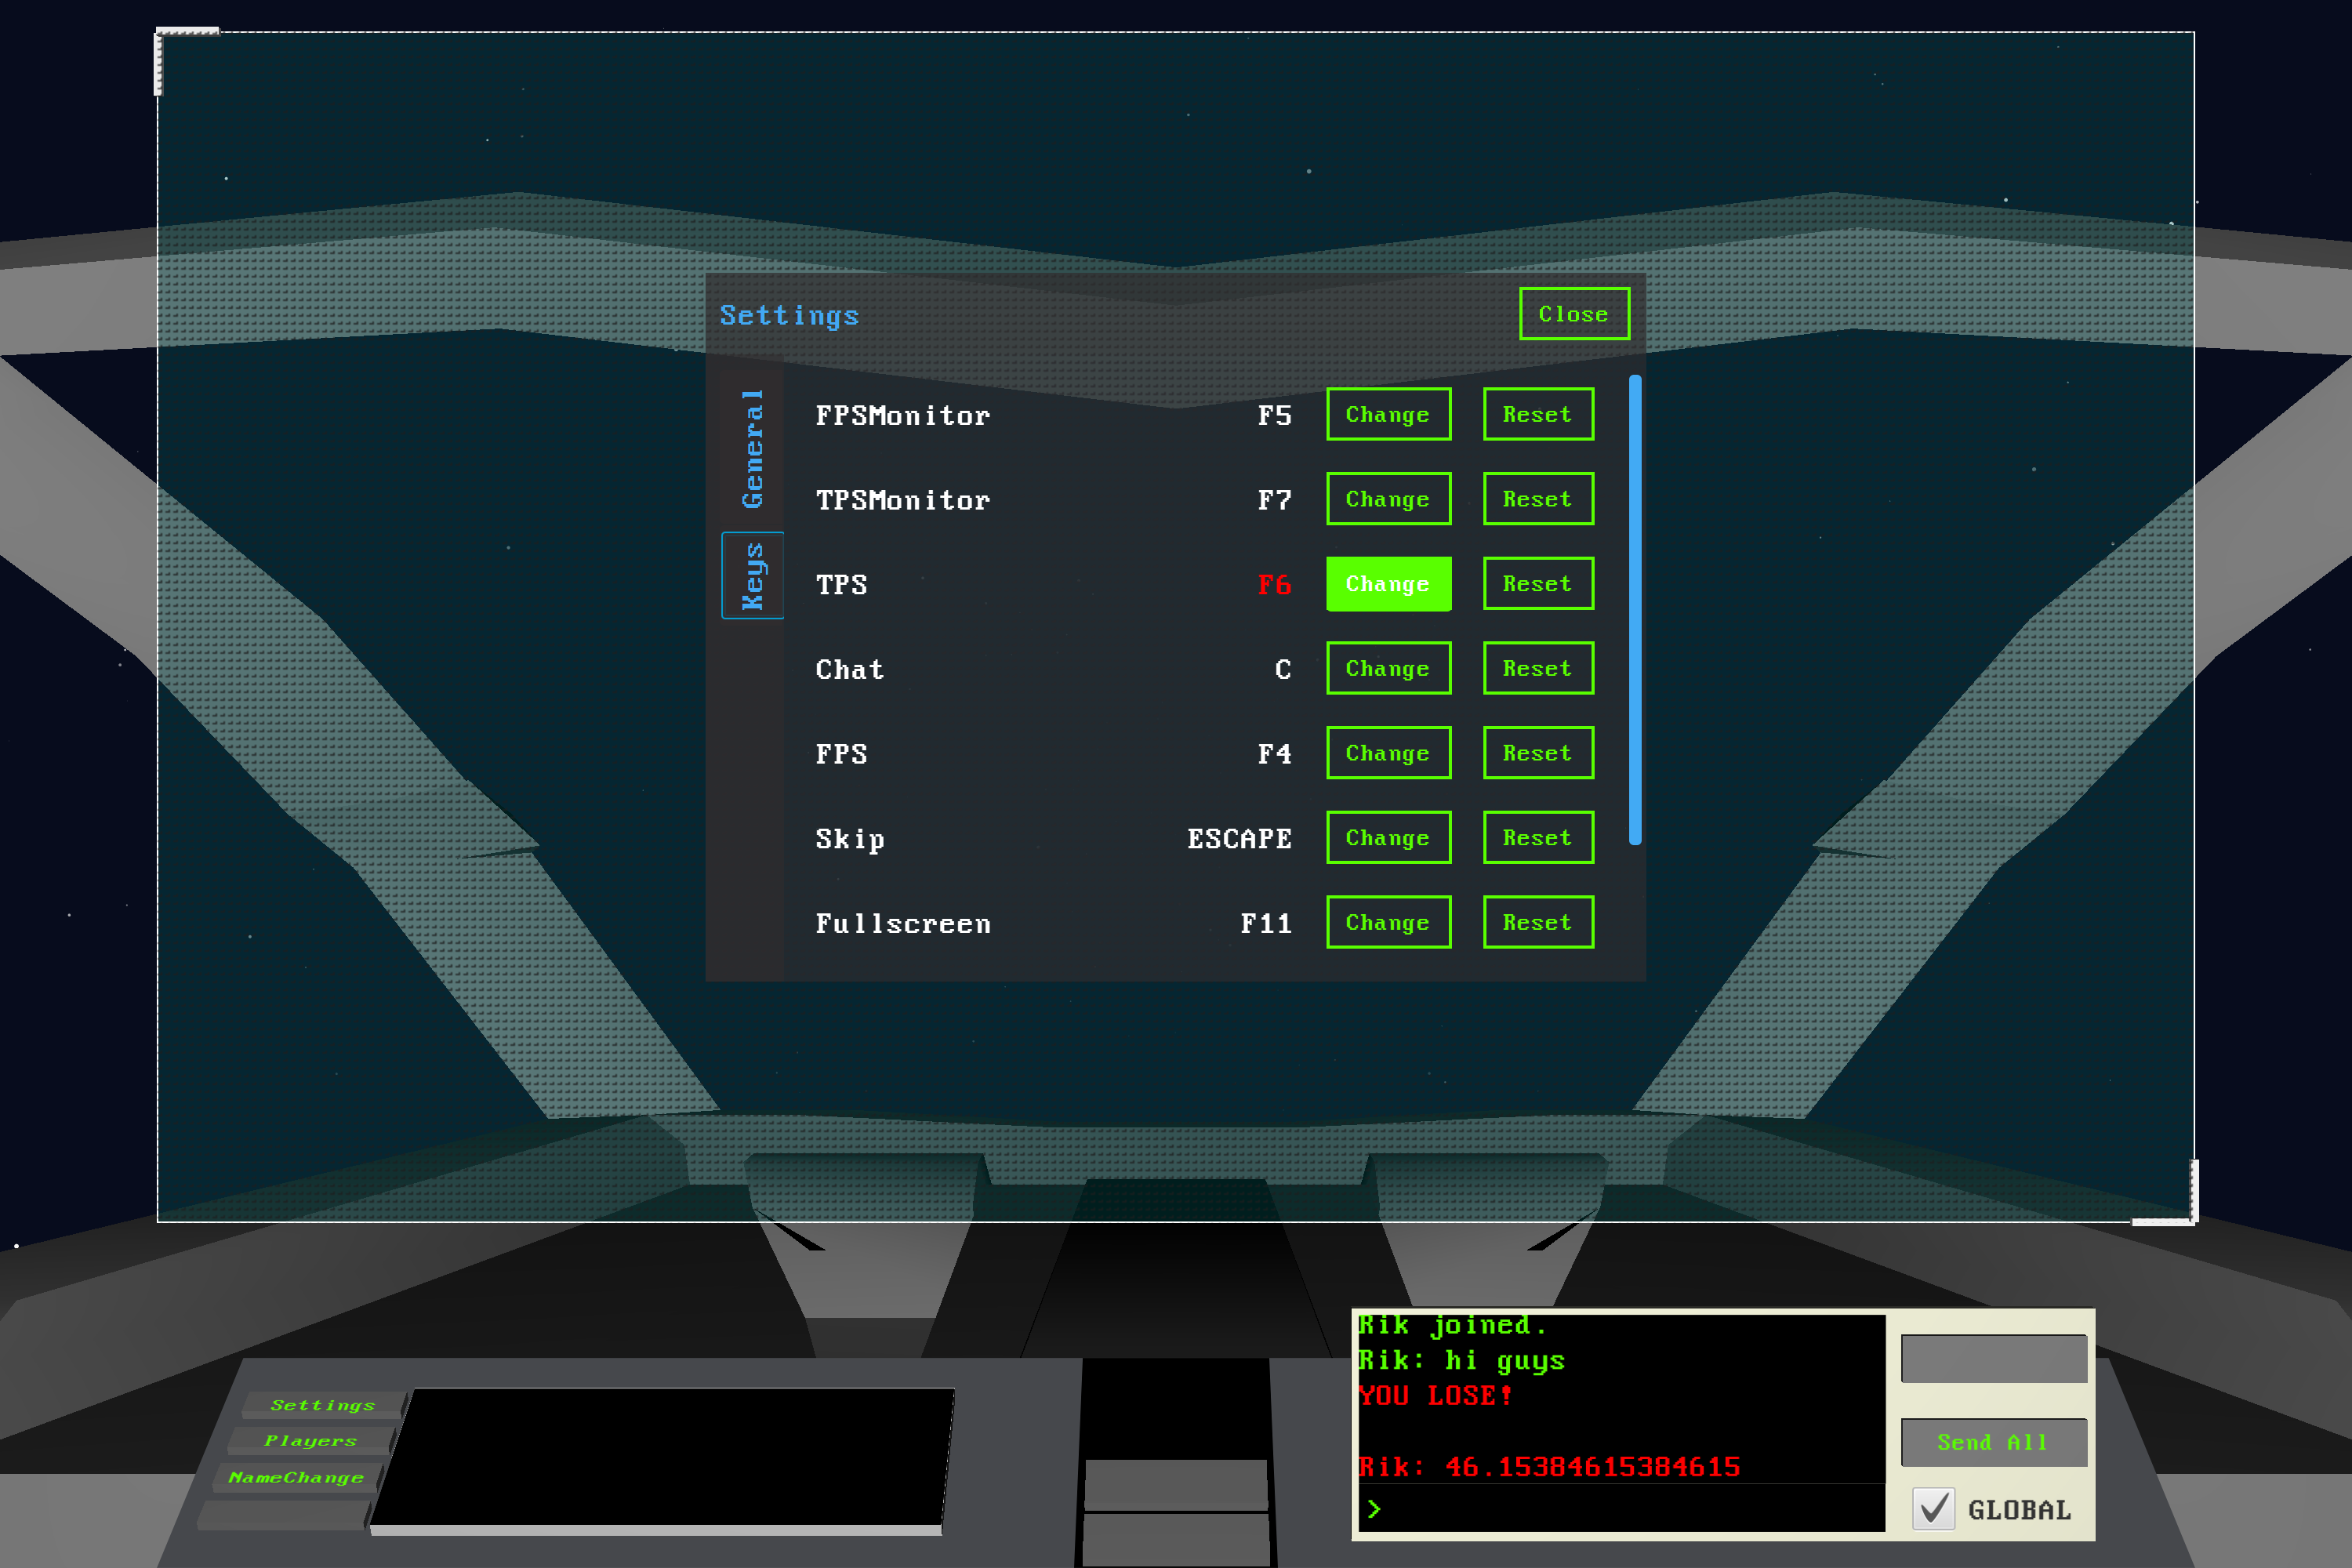
\includegraphics[width=.85\textwidth]{chapters/keybindings/keybinding.png}
  \caption*{Key Binding Menu}
\end{figure}
